% !TeX spellcheck = en_US
\chapter{System design} % Main chapter title

\label{chap:design} % Change X to a consecutive number; for referencing this chapter elsewhere, use \ref{ChapterX}

\lhead{Chapter \ref*{chap:design}. \emph{System design}} % Change X to a consecutive number; this is for the header on each page - perhaps a shortened title
Various applications for realizing the architecture have been compared. In the following sections the different options that were taken into account are presented.

\section{Orchestration engine}
Orchestration engines aggregate the processes and tools that are used to distribute services across mult\ac{IP}le machines. Further, mult\ac{IP}le replications are provided to maintain reliability. In addition, some solutions offer load balancing of incoming requests and network interconnection.
What all of these engines have in common is that a group of virtual machines or containers, known as "nodes", are managed from a central spot. An administrator directs what application is run on the cluster. Based on the application's metadata, the orchestration engine then decides where to run the application by selecting a node inside that cluster.

The engine of choice was \ac{K8s} because of its rich feature set.
Also studies showed that \ac{K8s} outperforms Docker Swarms when it comes to performance. For example, Marathe et.~al.~\cite{Marathe.2019} compared a simple web server service deployed on a Docker Swarm cluster with a \ac{K8s} cluster. The results showed better performance for \ac{K8s} in terms of memory consumption and CPU usage. Another study of Kang~et.~al.~\cite{Kang.2021} compared the performance of Docker Swarm and \ac{K8s} in a limited computing environment on Raspberry Pi boards. They also concluded that \ac{K8s} outperforms Docker Swarm if used with a high amount~(=30) of service containers on 3~Pi boards~\cite{Kang.2021}. Since they focused on container distribution and management methods this might get handy in the use case scenario under study.

\paragraph{Hyper-V Replication}
Microsoft Windows supports a replication mechanism for virtual machines hosted by Hyper-V. The existing virtual machines are mirrored to secondary virtual machine host servers which highers scalability and reliability. The replications are replicated to a secondary Hyper-V host server, enabling process continuity and recovery on outages.
Although there are benefits, like scalability and recovery, Hyper-V is mainly designed for virtual machines. Therefore, the cluster management solution is not applicable on this use case.

\paragraph{Docker Swarm}
"Docker Swarm" is a cluster and orchestration engine for the container service "Docker". The offered extension mode has more features compared to the Hyper-V replication and is specialized for containers. For example, Load Balancing, increased fault tolerance and automatic service discovery.
A highlighted feature among Docker Swarm is the decentralized design. That means, manager and application service can both run on any node within the cluster. Since it comes with Docker, no additional installation is required if Docker is already installed on the system.
However, since it is bound to the Docker API, using this orchestration technology involves the risk of inflexibility later on ("vendor lock-in").

%\paragraph{Open Shift}
%"Open Shift" is a application platform for clustering and orchestration of containers. It encapsulates \ac{K8s} and is similar to Kubernetes. It is also not free to use.
 
% andere sind mit Funktionsumfang sehr limitiert?
\paragraph{Kubernetes}
\acf{K8s} is a orchestration engine similar to "Docker Swarm". Load balancing, auto-scaling and automatic service discovery are also offered. However, \ac{K8s} additionally comes with the ability to rollback to a previous version in a product lifecycle and has built-in support for auto-scaling.
However, \ac{K8s} has more sophisticated configuration options which makes it harder to configure in the beginning.

\section{Kubernetes}
Since \ac{K8s} is the chosen orchestration engine, the following sections are taking a deeper look inside its architecture.

\subsection{Entities}
There are many entities for objects inside the cluster. For descr\ac{IP}tion of those entities the configuration language YAML is used. Some of the most widely used entities are described in the following paragraphs.
\paragraph{Deployment} Deployments are used to define declarative states for Pods. This allows to maintain consecutive versions of the pod and upgrade them during runtime.
\paragraph{Pod} A pod represents a set of running containers on a node. Each pod has additional information stored, such as Health state, the cluster internal network \ac{IP} address or the amoun of replications.
\paragraph{Daemon set} These ensure that mult\ac{IP}le (or all) nodes run a certain pod\cite{Kubernetes.20220831}. Common use cases are tasks for all nodes or running the network overlay pod.
\paragraph{User} This entity describes a user that  can acces the Kubernetes cluster and API services. Users can be part of a group and permission roles.
\paragraph{Node} A node represents a physical machine inside the cluster. Nodes can run mult\ac{IP}le pods.

\subsection{Services}
\ac{K8s} comes with a set of core services (see \autoref{fig.kubernetes-architecture}) that ensure the life span of scheduled containers, and the application services that offer the actual application.
\begin{figure}[h]
	\centering
	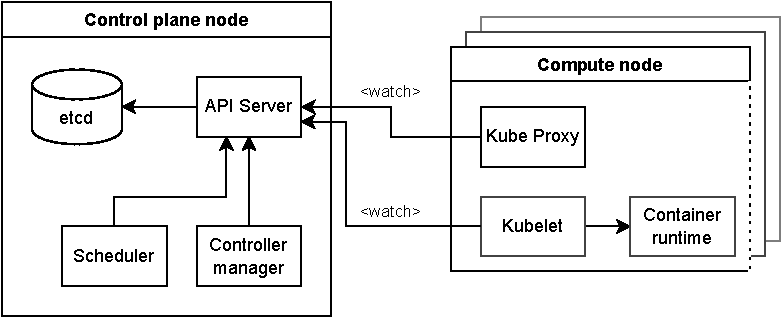
\includegraphics[width=0.75\textwidth]{Figures/kubernetes-architecture.pdf}
	\caption{Core and compute services for Kubernetes}
	\label{fig.kubernetes-architecture}
\end{figure}

In the following paragraphs, the crucial services are described in detail. Since every service is a pod, they can have mult\ac{IP}le replicas. Only the core service have to run on a dedicated Linux node the so called "control plane node". The other services can run on nodes for executing the applications and perform computations ("compute node").

\paragraph{etcd}
The etcd\footnote{etcd: https://etcd.io/} database server is a key-value store designed for distributed systems\cite{Luksa.2018}. That means it could run with mutl\ac{IP}le replications and would still be able to keep a persistent storage synchronized accross mult\ac{IP}le instances. It contains the applied configuration of several cluster entities (e.g. User configurations, deployments, pod configurations).

\paragraph{API server}
This is a RESTful web server that serves the Kubernetes API via HTTP\cite{Kubernetes.20221024}. It is the central joint between the services and establishes communication between users, external components and other core services. It makes the objects stored in etcd accessible over an Open API specification\cite{Luksa.2018,OpenAPIInitiative.20230210} and allows observing changes on the entities. The \ac{cli} tools "kubectl" and "kubeadm" both interact with the API server.

\paragraph{Kubelet} Kubelet is the service on the operating system level that maintains the pod life cycle and ensures the runtime of a container inside a pod. Furthermore, it manages the registration of the node to the control plane and reports its health and pod status to the API server.

\paragraph{Kube Proxy} The Kube-Proxy runs as a separate pod on every compute node. It maintains the connectivity between the services and pods\cite{Luksa.2018}. For a given \ac{IP} address and port combination it assures the connection to the corresponding pod. If mult\ac{IP}le pods can offer a service, the proxy also acts as a load balancer\cite{Luksa.2018}.

\paragraph{Scheduler} The scheduler is responsible for distributing services on the cluster and determining which node to choose during runtime. It reads conditions for scheduling (e.g. hardware resources, operating system, labels) from the API server and decides which node matches the configuration\cite{Luksa.2018}.

\paragraph{Controller manager} While the API-Server is responsible for storing data in etcd and announcing changes to the clients, the Controller manager and its parts try to achieve a described target state\cite{Luksa.2018}. The controller manager consists of several controllers for replications, daemon sets, deployments, volumes, and so on.


\subsection{Cluster networking}
Cluster networking is achieved using two components: The network plugin and the \ac{CNI}. Pods receive their own \ac{IP} address and can communicate with other pods. However, this is not a functionality which is achieved by Kubernetes directly. By using a \ac{CNI} the automated generation of network addresses and their inclusion is achieved when new containers are create or destroyed. It is crucial that pods share the same subnet across all the nodes in a cluster and \ac{NAT} is avoided\cite{Luksa.2018}.

Network plugins do implement the \ac{CNI}. They usually come with a manifest for a daemon set that introduces a network agent on all nodes inside the cluster to support the network communication.
For setting up the network interface, namespace and its \ac{IP} address, a dedicated container image is used. This is called the "pause container" image.

Even though, the team behind \ac{K8s} do not recommend any specific network plugin, there are only a few common network plugins widely used. For this case, Flannel is used as network plugin, since it is the described plugin used in the documentations for setting up \ac{K8s} with Windows containers\cite{GitHubKubernetesSIGWindowsTools.20230213,Kubernetes.20220419}. Hence, support for this \ac{CNI} plugin in relation with Windows containers is larger.

\paragraph{Flannel}
Flannel\footnote{Flannel: https://github.com/flannel-io/flannel} was originally developed as part from Fedora CoreOS\footnote{CoreOS: https://getfedora.org/en/coreos}\cite{SuseRancherCommunity.20230212}. It works with various backends for transferring packets in the internal network. Two possible backends are virtual extensible Local Area Network ("vxlan") and host gateway ("host-gw"). While "host-gw" needs an existing infrastructure and performs routing on the layer 3 network level, VXLAN is more flexible and could also be used in cloud environments\cite{GitHubFlannel.io.20230212}. VXLAN is an overlay protocol and encapsulates layer 2 Ethernet frames within datagrams\cite{SuseRancherCommunity.20230212}. It is similar to regular VLAN, but offers more than 4,096 network identifiers\cite{SuseRancherCommunity.20230212}. Thus, VXLAN is a good choice for highly scalable systems.

\paragraph{Calico}
Compared to Flannel, Calico\footnote{Tigera's Calico: https://www.tigera.io/project-calico/} is stated to be more performative, flexible and powerful\cite{SuseRancherCommunity.20230212,Tigera.20230210}. Calico comes with a sophisticated access control system\cite{Tigera.20230210} and more configuration options. However, its advanced configuration makes it hard to maintain long-term.

\section{Container environment}
The container environment (or "container runtime" (CRI)) runs the isolation layer between the physical host machine and the \ac{K8s} cluster by using containerization of processes.

While \ac{K8s} used to support the Docker-CRI as their standard container runtime, they announced it to be deprecated in 2020, and finally removed the support in February 2022\cite{Kubernetes.2020}. 
However, the specification for containerd's "Containerfile" has only minor differences compared to Docker's "Dockerfile". Thus, containerd files are fully compatible to docker files.

As container environment \tcode{containerd} is used. Containerd is..
In comparison to other container environments this is ...

At the current time being, container networking with containerd is not well-established on Windows~\cite{GitHub.20230202,GitHub.20230202b,Github.2022_258,GitHub.20230202c} even though docker-cri is already removed in current versions of \ac{K8s}~\cite{Kubernetes.2020}. However, these are the only two working container backends for Windows containers. Therefore containerd as container backend was chosen.

\paragraph{docker-cri}
\paragraph{containerd}
	- container runtime which is used in docker
	-> Only tech with support for Windows - equal tech stack everywhere
\paragraph{LXC container}
	linux containers



% Warum dieses Windows image?
% Windows Server Core and Nanoserver are the most common base images to target. The key difference between these images is that Nanoserver has a significantly smaller API surface. PowerShell, WMI, and the Windows servicing stack are absent from the Nanoserver image.
% Nanoserver was built to provide just enough API surface to run apps that have a dependency on .NET core or other modern open source frameworks. As a tradeoff to the smaller API surface, the Nanoserver image has a significantly smaller on-disk footprint than the rest of the Windows base images. Keep in mind that you can always add layers on top of Nano Server as you see fit. For an example of this check out the .NET Core Nano Server Dockerfile.
% Quelle: https://learn.microsoft.com/en-us/virtualization/windowscontainers/manage-containers/container-base-images



\section{Target architecture}
The application needs to be distributed on mult\ac{IP}le systems. Kubernetes supports application rollout only as container images. To be able to distribute the services on a cluster management tool a containerization of the application is necessary.